\chapter{Literature Review}
There are a total of twenty research articles that have been reviewed by us for the literature study that we have conducted. Some of them are directly associated with the creation of frequently asked questions, while others investigate string similarity and etc.

\pagebreak
\section{FAQ Processing}
FAQ retrieval is a crucial task when it comes to question answer pairs rankings \cite{faq_gen_1}. It is a process of retrieving the most relevant questions from a large collection of questions based on a user query. Achieving excellent performance in this task will solve many problems that we've discussed in the previous chapter \ref*{ch:problem_statement}. However, most of the traditional methods for FAQ generation are based on the use of extensive manual classification and engineering \cite{faq_gen_1}, this method takes tremendous amount of time and effort to be done. This was particularly highlighted by \cite{10.1007/978-3-319-18356-5_30} \cite{5615722} \cite{6227139} \cite{7817112} In addition, the performance of the system is also affected by the quality of the manual classification and engineering.

To address the issues brought-up, there are attempts and researches that have done to improve the situation. One of the approaches on solving the problem, is to automate the process of FAQ generation using NLP techniques. \cite{faq_gen_1} has made progress on using deep learning methods such as combining both Deep Matching Networks and Multihop Attention Networks in performing FAQ retrieval. Deep Matching Network also known as (DMN) is a deep learning model that generates a matching scores based of 2 matrices inputs. The matrices are made of the dot product of embeddings of every word of question with every word of answers.While Multihop Attention Networks on the other hand is proven to be effective for reasonings tasks like question answering, which is our focus in this paper \cite{faq_gen_1}. The network uses multiple "hops" of attention to gather information from a given input and make a prediction. It starts by encoding the input and then uses a decoder network that iteratively attends to different parts of the input, in order to generate an output.

\cite{10.1007/978-3-319-18356-5_30} takes an appraoch where a whole architecture is designed to achieve Auto-Faq-Gen which includes scraping, question construction, a ranking algorithm, and the question generation

\begin{figure}[H]
  \noindent 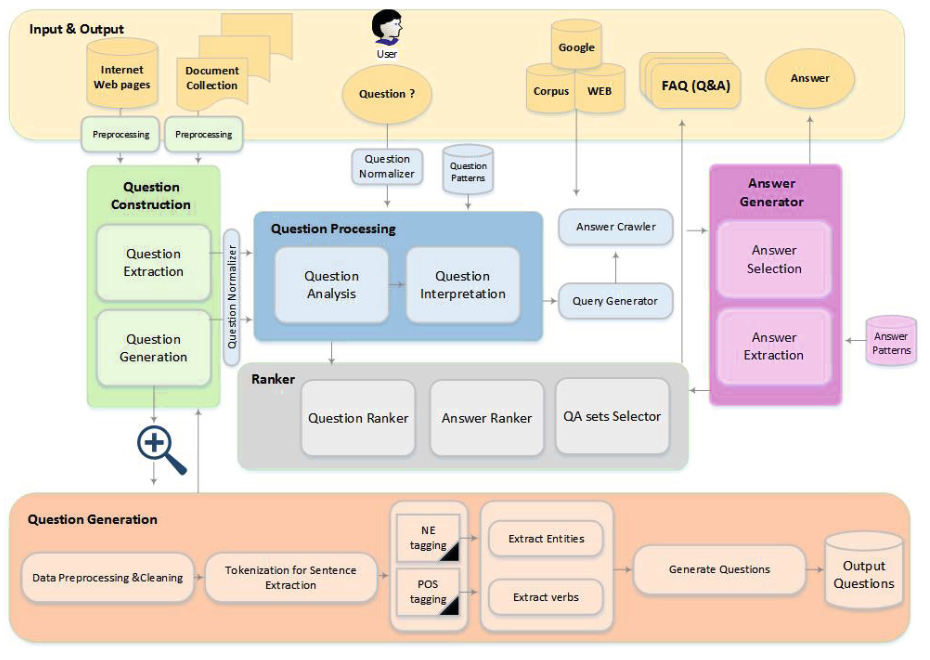
\includegraphics[scale=0.87]{assets/auto-faq-gen-architecture.png}
\caption{Auto FAQ Gen Architecture}\label{auto-faq-gen-arch}
\end{figure}

\pagebreak 
\section{Stop Words}
qwe

\pagebreak
\section{Similarity Matching}
\subsection*{Problem}
Another issue arises, where most of the time, the questions asked by the user might not be easily classified to fit with the existing questions in the FAQ database. This is because the questions asked by the user might be in a different form or context \cite{10.1007/978-3-319-42911-3_25}. For example, the question asked by the user might be in a different language, or the question asked by the user might be in a different form. 

Grammatically, misspellings are another set of issue that we can forsee when it comes to building automated questions answerings, highlighted by \cite{sms_faq_retrieval}.

\pagebreak
\subsection*{Solution}
Similarity Matching is important when it comes to ranking the answers to the user query. The traditional way to score similarity is naive, where the score is calculated by levenshtein distance. \cite{8054419} However, this method is not effective when it comes to ranking the answers. This is because the levenshtein distance is not able to capture the semantic meaning of the words. Another concept comes to mind which is BOW, the bag of words model, \cite{Improving_question_retrieval_in_community_question_answering_using_world_knowledge} highlighted to us where, BOWs similarity matching algorithm can be used on processed text (stop words removal, stemming, etc) to calculate the similarity between the query and the answer, however similarly to levenshtein distance, BOWs is not able to capture the semantic meaning of the words, which will bring false conceptual similarity between the query and the answer.

Word knowledge or Word Embedding is one of the solution to the traditional similarity matching algorithm. \cite{Improving_question_retrieval_in_community_question_answering_using_world_knowledge} proposed a method that uses word knowledge to improve the similarity matching algorithm. The model stitch together a knowledge base to a word, which then constructs a knowledge table which consists of the raw words, Hypernyms, Synonyms and Associative concept of words. This solution breaks the traditional similarity matching algorithm, where the similarity is calculated by the semantic meaning of the words, instead of the raw words. \cite{OTHMAN2019485} has made progress on proposing a method called "WEKOS (Word Embedding, Kmeans
and COSine based method)". WEKOS (Word Embedding, Kmeans and COSine) is a new method for question retrieval. The word embeddings of a question are weighted and averaged to get an overall representation of the question. The continuous word representations are learned in advance using the continuous bag-of-words (CBOW) model. \cite{OTHMAN2019485} The cosine similarity is used to calculate the similarity between the average of the word vectors corresponding to the question and that of each existing question.

\section{FAQ Rankings}
Deep Matching Network also known as (DMN) is a deep learning model that generates a matching scores based of 2 matrices inputs. The matrices are made of the dot product of embeddings of every word of question with every word of answers.

Multi-hop Attention Network on the other hand is proven to be effective for reasonings tasks like question answering, which is our focus in this paper \cite{faq_gen_1}. The network uses multiple "hops" of attention to gather information from a given input and make a prediction. It starts by encoding the input and then uses a decoder network that iteratively attends to different parts of the input, in order to generate an output.

In order to solve the issue of context misconception between the query and the faq. We can highlight the issue below. 

\begin{figure}[H]
  \centering
  \noindent 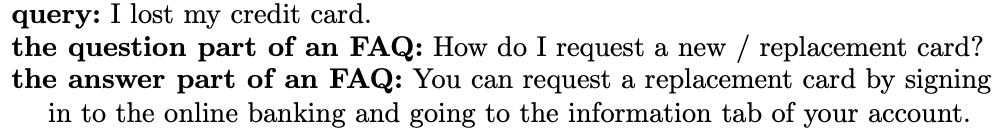
\includegraphics[scale=0.85]{assets/An_FAQ_search_method_query_issue.png}
\caption{Misconception}\label{misconception_1}
\end{figure}

In the above example \ref*{misconception_1}, the query only matched with the correct output with 2 characters "I" and "Card", that way, the resulting score will be very low, even though the FAQ is relevant to the query. To counter this issue, the authors of \cite{10.1007/978-3-319-42911-3_25} proposed a method that predicts if the query corresponds to a FAQ using document classifier. The paper begins to highlight that the proposed document classifier uses binary classifiers to classifier each faq to the query. The sentences are broken into unigrams, bigrams to learn the dependency relation between the query and the faq.

\pagebreak

\section{Sentiment Analysis}
qwe

\pagebreak
\section{Summarization}
Text summarization is the process of automatically generating a shorter version of a text that preserves the most important information. There are two main types of text summarization: extractive and abstractive. Extractive summarization involves selecting and concatenating important sentences from the original text, while abstractive summarization involves generating new sentences that summarize the meaning of the original text.

One of the earliest and most influential papers in the field of text summarization is "Automatic Text Summarization" by Edmund H. H. Hovy and Eduard Hovy (2003). This paper provides a comprehensive overview of the history, current state, and future directions of text summarization research.

Another important paper in the field is "A Survey of Text Summarization Techniques" by Inderjeet Mani and Mark T. Maybury (2001). This paper provides a detailed survey of the different techniques used in extractive and abstractive summarization, as well as an evaluation of their strengths and weaknesses.

Other notable papers include "Abstractive Text Summarization Using Sequence to Sequence RNNs and Beyond" by Alexander Rush et al (2015) which proposed the use of sequence to sequence neural networks for abstractive summarization and "Get To The Point: Summarization with Pointer Generator Networks" by Abigail See et al (2017) that proposed the pointer generator network for abstractive summarization.

\section{Evaluation Metrics}
qwe
